\documentclass[1p]{elsarticle_modified}
%\bibliographystyle{elsarticle-num}

%\usepackage[colorlinks]{hyperref}
%\usepackage{abbrmath_seonhwa} %\Abb, \Ascr, \Acal ,\Abf, \Afrak
\usepackage{amsfonts}
\usepackage{amssymb}
\usepackage{amsmath}
\usepackage{amsthm}
\usepackage{scalefnt}
\usepackage{amsbsy}
\usepackage{kotex}
\usepackage{caption}
\usepackage{subfig}
\usepackage{color}
\usepackage{graphicx}
\usepackage{xcolor} %% white, black, red, green, blue, cyan, magenta, yellow
\usepackage{float}
\usepackage{setspace}
\usepackage{hyperref}

\usepackage{tikz}
\usetikzlibrary{arrows}

\usepackage{multirow}
\usepackage{array} % fixed length table
\usepackage{hhline}

%%%%%%%%%%%%%%%%%%%%%
\makeatletter
\renewcommand*\env@matrix[1][\arraystretch]{%
	\edef\arraystretch{#1}%
	\hskip -\arraycolsep
	\let\@ifnextchar\new@ifnextchar
	\array{*\c@MaxMatrixCols c}}
\makeatother %https://tex.stackexchange.com/questions/14071/how-can-i-increase-the-line-spacing-in-a-matrix
%%%%%%%%%%%%%%%

\usepackage[normalem]{ulem}

\newcommand{\msout}[1]{\ifmmode\text{\sout{\ensuremath{#1}}}\else\sout{#1}\fi}
%SOURCE: \msout is \stkout macro in https://tex.stackexchange.com/questions/20609/strikeout-in-math-mode

\newcommand{\cancel}[1]{
	\ifmmode
	{\color{red}\msout{#1}}
	\else
	{\color{red}\sout{#1}}
	\fi
}

\newcommand{\add}[1]{
	{\color{blue}\uwave{#1}}
}

\newcommand{\replace}[2]{
	\ifmmode
	{\color{red}\msout{#1}}{\color{blue}\uwave{#2}}
	\else
	{\color{red}\sout{#1}}{\color{blue}\uwave{#2}}
	\fi
}

\newcommand{\Sol}{\mathcal{S}} %segment
\newcommand{\D}{D} %diagram
\newcommand{\A}{\mathcal{A}} %arc


%%%%%%%%%%%%%%%%%%%%%%%%%%%%%5 test

\def\sl{\operatorname{\textup{SL}}(2,\Cbb)}
\def\psl{\operatorname{\textup{PSL}}(2,\Cbb)}
\def\quan{\mkern 1mu \triangleright \mkern 1mu}

\theoremstyle{definition}
\newtheorem{thm}{Theorem}[section]
\newtheorem{prop}[thm]{Proposition}
\newtheorem{lem}[thm]{Lemma}
\newtheorem{ques}[thm]{Question}
\newtheorem{cor}[thm]{Corollary}
\newtheorem{defn}[thm]{Definition}
\newtheorem{exam}[thm]{Example}
\newtheorem{rmk}[thm]{Remark}
\newtheorem{alg}[thm]{Algorithm}

\newcommand{\I}{\sqrt{-1}}
\begin{document}

%\begin{frontmatter}
%
%\title{Boundary parabolic representations of knots up to 8 crossings}
%
%%% Group authors per affiliation:
%\author{Yunhi Cho} 
%\address{Department of Mathematics, University of Seoul, Seoul, Korea}
%\ead{yhcho@uos.ac.kr}
%
%
%\author{Seonhwa Kim} %\fnref{s_kim}}
%\address{Center for Geometry and Physics, Institute for Basic Science, Pohang, 37673, Korea}
%\ead{ryeona17@ibs.re.kr}
%
%\author{Hyuk Kim}
%\address{Department of Mathematical Sciences, Seoul National University, Seoul 08826, Korea}
%\ead{hyukkim@snu.ac.kr}
%
%\author{Seokbeom Yoon}
%\address{Department of Mathematical Sciences, Seoul National University, Seoul, 08826,  Korea}
%\ead{sbyoon15@snu.ac.kr}
%
%\begin{abstract}
%We find all boundary parabolic representation of knots up to 8 crossings.
%
%\end{abstract}
%\begin{keyword}
%    \MSC[2010] 57M25 
%\end{keyword}
%
%\end{frontmatter}

%\linenumbers
%\tableofcontents
%
\newcommand\colored[1]{\textcolor{white}{\rule[-0.35ex]{0.8em}{1.4ex}}\kern-0.8em\color{red} #1}%
%\newcommand\colored[1]{\textcolor{white}{ #1}\kern-2.17ex	\textcolor{white}{ #1}\kern-1.81ex	\textcolor{white}{ #1}\kern-2.15ex\color{red}#1	}

{\Large $\underline{12n_{0188}~(K12n_{0188})}$}

\setlength{\tabcolsep}{10pt}
\renewcommand{\arraystretch}{1.6}
\vspace{1cm}\begin{tabular}{m{100pt}>{\centering\arraybackslash}m{274pt}}
\multirow{5}{120pt}{
	\centering
	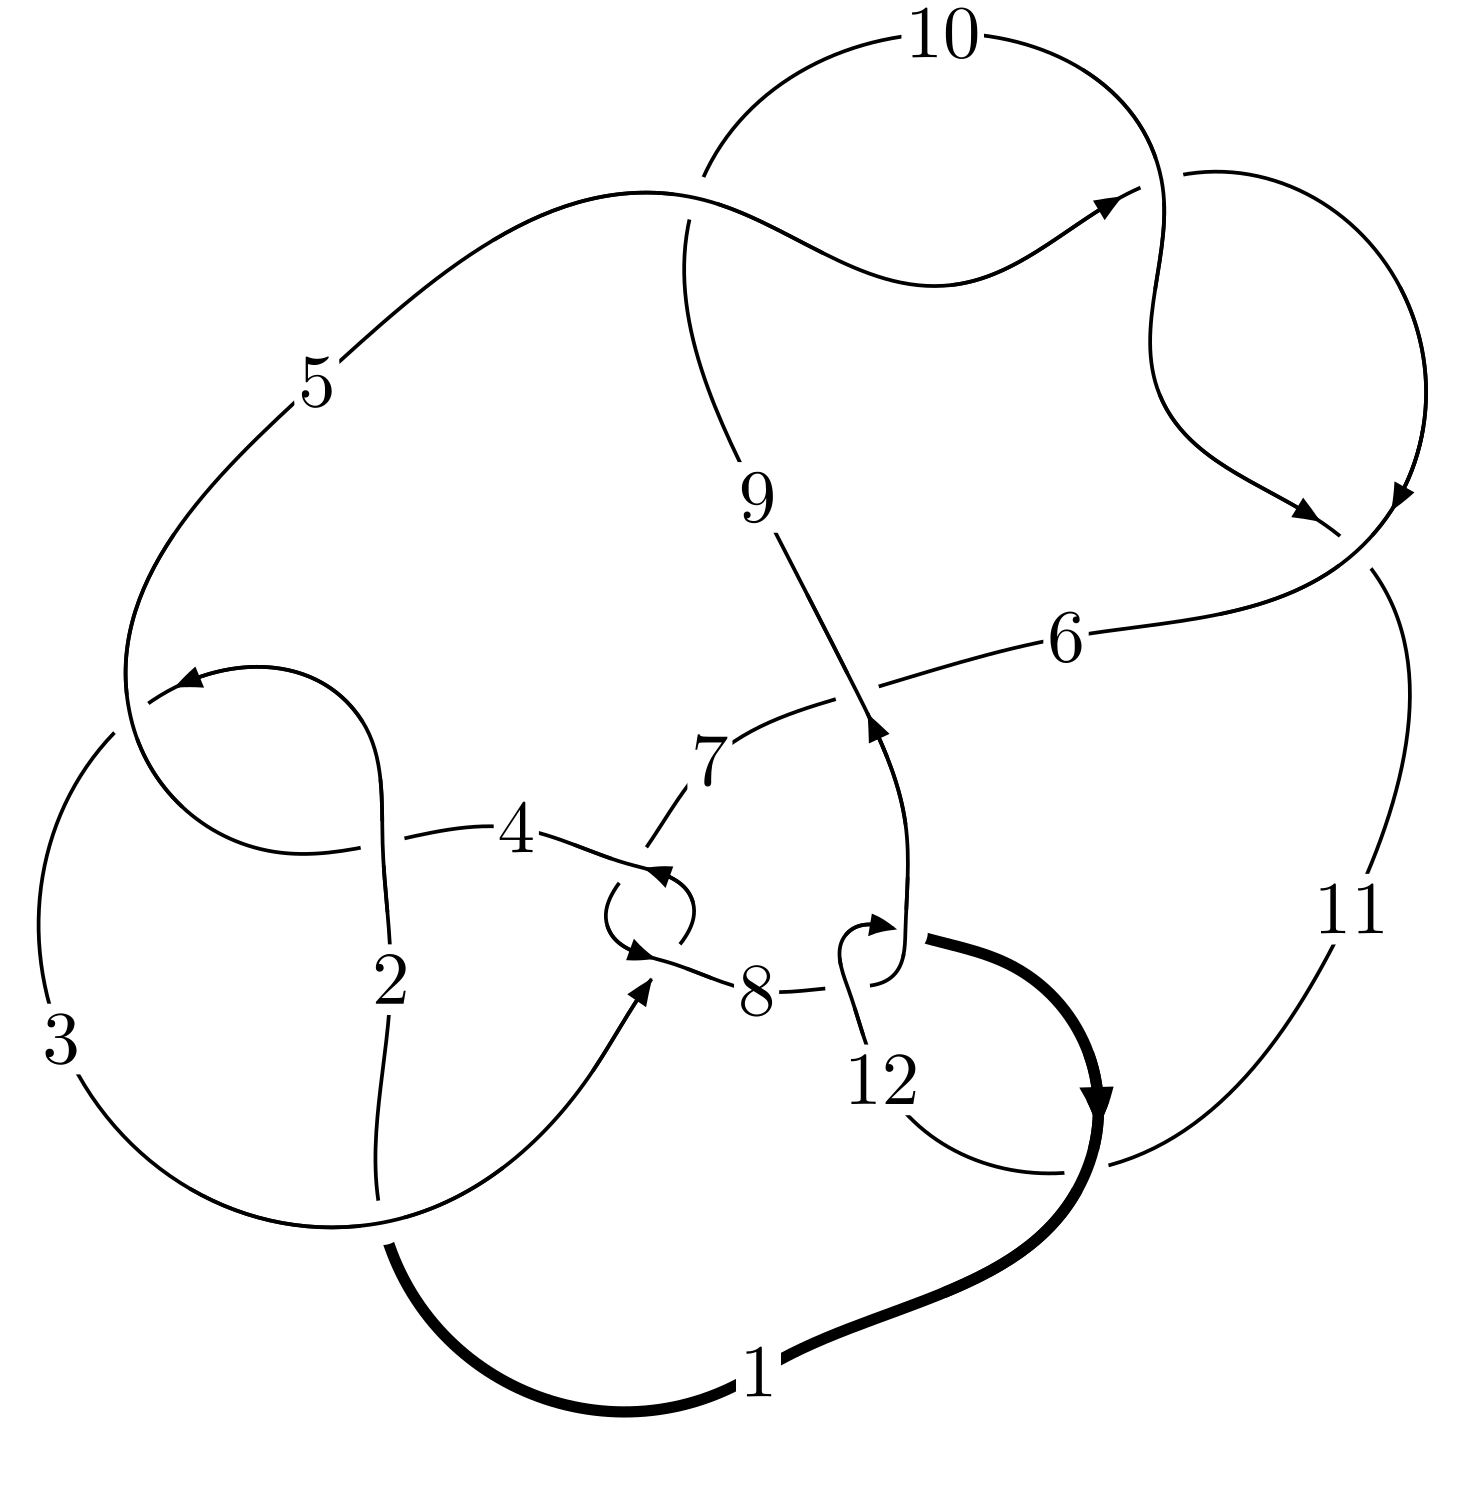
\includegraphics[width=112pt]{../../../GIT/diagram.site/Diagrams/png/2277_12n_0188.png}\\
\ \ \ A knot diagram\footnotemark}&
\allowdisplaybreaks
\textbf{Linearized knot diagam} \\
\cline{2-2}
 &
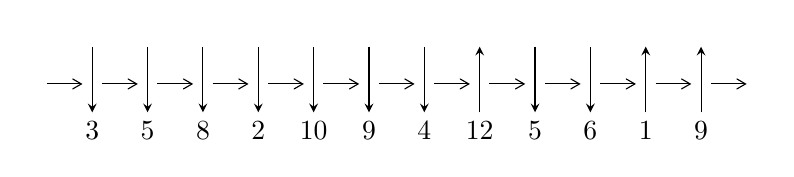
\begin{tikzpicture}[x=20pt, y=17pt]
	% nodes
	\node (C0) at (0, 0) {};
	\node (C1) at (1, 0) {};
	\node (C1U) at (1, +1) {};
	\node (C1D) at (1, -1) {3};

	\node (C2) at (2, 0) {};
	\node (C2U) at (2, +1) {};
	\node (C2D) at (2, -1) {5};

	\node (C3) at (3, 0) {};
	\node (C3U) at (3, +1) {};
	\node (C3D) at (3, -1) {8};

	\node (C4) at (4, 0) {};
	\node (C4U) at (4, +1) {};
	\node (C4D) at (4, -1) {2};

	\node (C5) at (5, 0) {};
	\node (C5U) at (5, +1) {};
	\node (C5D) at (5, -1) {10};

	\node (C6) at (6, 0) {};
	\node (C6U) at (6, +1) {};
	\node (C6D) at (6, -1) {9};

	\node (C7) at (7, 0) {};
	\node (C7U) at (7, +1) {};
	\node (C7D) at (7, -1) {4};

	\node (C8) at (8, 0) {};
	\node (C8U) at (8, +1) {};
	\node (C8D) at (8, -1) {12};

	\node (C9) at (9, 0) {};
	\node (C9U) at (9, +1) {};
	\node (C9D) at (9, -1) {5};

	\node (C10) at (10, 0) {};
	\node (C10U) at (10, +1) {};
	\node (C10D) at (10, -1) {6};

	\node (C11) at (11, 0) {};
	\node (C11U) at (11, +1) {};
	\node (C11D) at (11, -1) {1};

	\node (C12) at (12, 0) {};
	\node (C12U) at (12, +1) {};
	\node (C12D) at (12, -1) {9};
	\node (C13) at (13, 0) {};

	% arrows
	\draw[->,>={angle 60}]
	(C0) edge (C1) (C1) edge (C2) (C2) edge (C3) (C3) edge (C4) (C4) edge (C5) (C5) edge (C6) (C6) edge (C7) (C7) edge (C8) (C8) edge (C9) (C9) edge (C10) (C10) edge (C11) (C11) edge (C12) (C12) edge (C13) ;	\draw[->,>=stealth]
	(C1U) edge (C1D) (C2U) edge (C2D) (C3U) edge (C3D) (C4U) edge (C4D) (C5U) edge (C5D) (C6U) edge (C6D) (C7U) edge (C7D) (C8D) edge (C8U) (C9U) edge (C9D) (C10U) edge (C10D) (C11D) edge (C11U) (C12D) edge (C12U) ;
	\end{tikzpicture} \\
\hhline{~~} \\& 
\textbf{Solving Sequence} \\ \cline{2-2} 
 &
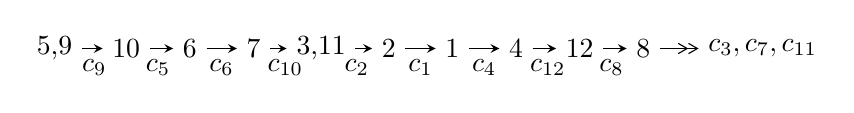
\begin{tikzpicture}[x=23pt, y=7pt]
	% node
	\node (A0) at (-1/8, 0) {5,9};
	\node (A1) at (1, 0) {10};
	\node (A2) at (2, 0) {6};
	\node (A3) at (3, 0) {7};
	\node (A4) at (65/16, 0) {3,11};
	\node (A5) at (41/8, 0) {2};
	\node (A6) at (49/8, 0) {1};
	\node (A7) at (57/8, 0) {4};
	\node (A8) at (65/8, 0) {12};
	\node (A9) at (73/8, 0) {8};
	\node (C1) at (1/2, -1) {$c_{9}$};
	\node (C2) at (3/2, -1) {$c_{5}$};
	\node (C3) at (5/2, -1) {$c_{6}$};
	\node (C4) at (7/2, -1) {$c_{10}$};
	\node (C5) at (37/8, -1) {$c_{2}$};
	\node (C6) at (45/8, -1) {$c_{1}$};
	\node (C7) at (53/8, -1) {$c_{4}$};
	\node (C8) at (61/8, -1) {$c_{12}$};
	\node (C9) at (69/8, -1) {$c_{8}$};
	\node (A10) at (11, 0) {$c_{3},c_{7},c_{11}$};

	% edge
	\draw[->,>=stealth]	
	(A0) edge (A1) (A1) edge (A2) (A2) edge (A3) (A3) edge (A4) (A4) edge (A5) (A5) edge (A6) (A6) edge (A7) (A7) edge (A8) (A8) edge (A9) ;
	\draw[->>,>={angle 60}]	
	(A9) edge (A10);
\end{tikzpicture} \\ 

\end{tabular} \\

\footnotetext{
The image of knot diagram is generated by the software ``\textbf{Draw programme}" developed by Andrew Bartholomew(\url{http://www.layer8.co.uk/maths/draw/index.htm\#Running-draw}), where we modified some parts for our purpose(\url{https://github.com/CATsTAILs/LinksPainter}).
}\phantom \\ \newline 
\centering \textbf{Ideals for irreducible components\footnotemark of $X_{\text{par}}$} 
 
\begin{align*}
I^u_{1}&=\langle 
1.51544\times10^{40} u^{40}+2.56027\times10^{40} u^{39}+\cdots+1.06321\times10^{41} b+4.21643\times10^{41},\\
\phantom{I^u_{1}}&\phantom{= \langle  }6.97778\times10^{40} u^{40}+1.95337\times10^{41} u^{39}+\cdots+2.12642\times10^{41} a-9.27571\times10^{40},\;u^{41}+3 u^{40}+\cdots-8 u-8\rangle \\
I^u_{2}&=\langle 
-2 a^2- a u+b-2 a- u-1,\;4 a^3+2 a^2 u- u,\;u^2-2\rangle \\
\\
I^v_{1}&=\langle 
a,\;b+v+2,\;v^3+3 v^2+2 v-1\rangle \\
\end{align*}
\raggedright * 3 irreducible components of $\dim_{\mathbb{C}}=0$, with total 50 representations.\\
\footnotetext{All coefficients of polynomials are rational numbers. But the coefficients are sometimes approximated in decimal forms when there is not enough margin.}
\newpage
\renewcommand{\arraystretch}{1}
\centering \section*{I. $I^u_{1}= \langle 1.52\times10^{40} u^{40}+2.56\times10^{40} u^{39}+\cdots+1.06\times10^{41} b+4.22\times10^{41},\;6.98\times10^{40} u^{40}+1.95\times10^{41} u^{39}+\cdots+2.13\times10^{41} a-9.28\times10^{40},\;u^{41}+3 u^{40}+\cdots-8 u-8 \rangle$}
\flushleft \textbf{(i) Arc colorings}\\
\begin{tabular}{m{7pt} m{180pt} m{7pt} m{180pt} }
\flushright $a_{5}=$&$\begin{pmatrix}0\\u\end{pmatrix}$ \\
\flushright $a_{9}=$&$\begin{pmatrix}1\\0\end{pmatrix}$ \\
\flushright $a_{10}=$&$\begin{pmatrix}1\\u^2\end{pmatrix}$ \\
\flushright $a_{6}=$&$\begin{pmatrix}- u\\- u^3+u\end{pmatrix}$ \\
\flushright $a_{7}=$&$\begin{pmatrix}u^3-2 u\\- u^3+u\end{pmatrix}$ \\
\flushright $a_{3}=$&$\begin{pmatrix}-0.328147 u^{40}-0.918618 u^{39}+\cdots-19.5503 u+0.436213\\-0.142535 u^{40}-0.240806 u^{39}+\cdots+7.40030 u-3.96576\end{pmatrix}$ \\
\flushright $a_{11}=$&$\begin{pmatrix}- u^2+1\\- u^4+2 u^2\end{pmatrix}$ \\
\flushright $a_{2}=$&$\begin{pmatrix}-0.328147 u^{40}-0.918618 u^{39}+\cdots-19.5503 u+0.436213\\0.0824090 u^{40}+0.163606 u^{39}+\cdots+9.49889 u-4.49235\end{pmatrix}$ \\
\flushright $a_{1}=$&$\begin{pmatrix}0.0838694 u^{40}+0.525518 u^{39}+\cdots+23.3356 u+7.39263\\-0.124059 u^{40}-0.154000 u^{39}+\cdots+5.97827 u+0.0223382\end{pmatrix}$ \\
\flushright $a_{4}=$&$\begin{pmatrix}-0.340779 u^{40}-1.11522 u^{39}+\cdots-14.5840 u-9.80822\\0.0747081 u^{40}-0.0614080 u^{39}+\cdots-12.3801 u+1.21809\end{pmatrix}$ \\
\flushright $a_{12}=$&$\begin{pmatrix}0.207928 u^{40}+0.679518 u^{39}+\cdots+17.3573 u+7.37029\\-0.124059 u^{40}-0.154000 u^{39}+\cdots+5.97827 u+0.0223382\end{pmatrix}$ \\
\flushright $a_{8}=$&$\begin{pmatrix}0.401561 u^{40}+1.01803 u^{39}+\cdots+27.2274 u+2.78868\\-0.142281 u^{40}-0.206934 u^{39}+\cdots-0.775735 u+2.43501\end{pmatrix}$\\&\end{tabular}
\flushleft \textbf{(ii) Obstruction class $= -1$}\\~\\
\flushleft \textbf{(iii) Cusp Shapes $= -0.588415 u^{40}-0.804243 u^{39}+\cdots+87.6228 u-60.0034$}\\~\\
\newpage\renewcommand{\arraystretch}{1}
\flushleft \textbf{(iv) u-Polynomials at the component}\newline \\
\begin{tabular}{m{50pt}|m{274pt}}
Crossings & \hspace{64pt}u-Polynomials at each crossing \\
\hline $$\begin{aligned}c_{1}\end{aligned}$$&$\begin{aligned}
&u^{41}+26 u^{40}+\cdots+206 u+1
\end{aligned}$\\
\hline $$\begin{aligned}c_{2},c_{4}\end{aligned}$$&$\begin{aligned}
&u^{41}-4 u^{40}+\cdots-14 u-1
\end{aligned}$\\
\hline $$\begin{aligned}c_{3},c_{7}\end{aligned}$$&$\begin{aligned}
&u^{41}+2 u^{40}+\cdots+8 u-1
\end{aligned}$\\
\hline $$\begin{aligned}c_{5},c_{9},c_{10}\end{aligned}$$&$\begin{aligned}
&u^{41}+3 u^{40}+\cdots-8 u-8
\end{aligned}$\\
\hline $$\begin{aligned}c_{6}\end{aligned}$$&$\begin{aligned}
&u^{41}-9 u^{40}+\cdots+10824 u+12200
\end{aligned}$\\
\hline $$\begin{aligned}c_{8},c_{12}\end{aligned}$$&$\begin{aligned}
&u^{41}-4 u^{40}+\cdots+5 u-7
\end{aligned}$\\
\hline $$\begin{aligned}c_{11}\end{aligned}$$&$\begin{aligned}
&u^{41}-12 u^{40}+\cdots+1593 u-49
\end{aligned}$\\
\hline
\end{tabular}\\~\\
\newpage\renewcommand{\arraystretch}{1}
\flushleft \textbf{(v) Riley Polynomials at the component}\newline \\
\begin{tabular}{m{50pt}|m{274pt}}
Crossings & \hspace{64pt}Riley Polynomials at each crossing \\
\hline $$\begin{aligned}c_{1}\end{aligned}$$&$\begin{aligned}
&y^{41}-18 y^{40}+\cdots+44086 y-1
\end{aligned}$\\
\hline $$\begin{aligned}c_{2},c_{4}\end{aligned}$$&$\begin{aligned}
&y^{41}-26 y^{40}+\cdots+206 y-1
\end{aligned}$\\
\hline $$\begin{aligned}c_{3},c_{7}\end{aligned}$$&$\begin{aligned}
&y^{41}+6 y^{40}+\cdots+54 y-1
\end{aligned}$\\
\hline $$\begin{aligned}c_{5},c_{9},c_{10}\end{aligned}$$&$\begin{aligned}
&y^{41}-55 y^{40}+\cdots+2752 y-64
\end{aligned}$\\
\hline $$\begin{aligned}c_{6}\end{aligned}$$&$\begin{aligned}
&y^{41}-139 y^{40}+\cdots+8334688576 y-148840000
\end{aligned}$\\
\hline $$\begin{aligned}c_{8},c_{12}\end{aligned}$$&$\begin{aligned}
&y^{41}-12 y^{40}+\cdots+1593 y-49
\end{aligned}$\\
\hline $$\begin{aligned}c_{11}\end{aligned}$$&$\begin{aligned}
&y^{41}+44 y^{40}+\cdots+664281 y-2401
\end{aligned}$\\
\hline
\end{tabular}\\~\\
\newpage\flushleft \textbf{(vi) Complex Volumes and Cusp Shapes}
$$\begin{array}{c|c|c}  
\text{Solutions to }I^u_{1}& \I (\text{vol} + \sqrt{-1}CS) & \text{Cusp shape}\\
 \hline 
\begin{aligned}
u &= \phantom{-}0.852625 + 0.482864 I \\
a &= -0.372803 - 0.780038 I \\
b &= \phantom{-}0.771778 - 0.848460 I\end{aligned}
 & -0.75167 - 5.04176 I & -5.33106 + 6.16840 I \\ \hline\begin{aligned}
u &= \phantom{-}0.852625 - 0.482864 I \\
a &= -0.372803 + 0.780038 I \\
b &= \phantom{-}0.771778 + 0.848460 I\end{aligned}
 & -0.75167 + 5.04176 I & -5.33106 - 6.16840 I \\ \hline\begin{aligned}
u &= -0.003882 + 1.032070 I \\
a &= -0.244627 - 1.101450 I \\
b &= \phantom{-}0.500255 + 0.850150 I\end{aligned}
 & -1.61122 + 4.08215 I & -8.92321 - 7.89693 I \\ \hline\begin{aligned}
u &= -0.003882 - 1.032070 I \\
a &= -0.244627 + 1.101450 I \\
b &= \phantom{-}0.500255 - 0.850150 I\end{aligned}
 & -1.61122 - 4.08215 I & -8.92321 + 7.89693 I \\ \hline\begin{aligned}
u &= -0.992946 + 0.343746 I \\
a &= \phantom{-}1.196560 + 0.016956 I \\
b &= -0.60773 - 1.75136 I\end{aligned}
 & -4.56663 + 3.64468 I & -10.21223 - 4.25500 I \\ \hline\begin{aligned}
u &= -0.992946 - 0.343746 I \\
a &= \phantom{-}1.196560 - 0.016956 I \\
b &= -0.60773 + 1.75136 I\end{aligned}
 & -4.56663 - 3.64468 I & -10.21223 + 4.25500 I \\ \hline\begin{aligned}
u &= \phantom{-}1.044990 + 0.164135 I \\
a &= -1.029770 + 0.479582 I \\
b &= -0.335570 + 0.883151 I\end{aligned}
 & -4.59839 - 1.02943 I & -11.04507 + 3.64044 I \\ \hline\begin{aligned}
u &= \phantom{-}1.044990 - 0.164135 I \\
a &= -1.029770 - 0.479582 I \\
b &= -0.335570 - 0.883151 I\end{aligned}
 & -4.59839 + 1.02943 I & -11.04507 - 3.64044 I \\ \hline\begin{aligned}
u &= -0.848129 + 0.093318 I \\
a &= \phantom{-}0.256235 - 0.617893 I \\
b &= \phantom{-}0.429896 - 0.866899 I\end{aligned}
 & -1.53932 + 0.15416 I & -7.41256 - 0.66382 I \\ \hline\begin{aligned}
u &= -0.848129 - 0.093318 I \\
a &= \phantom{-}0.256235 + 0.617893 I \\
b &= \phantom{-}0.429896 + 0.866899 I\end{aligned}
 & -1.53932 - 0.15416 I & -7.41256 + 0.66382 I\\
 \hline 
 \end{array}$$\newpage$$\begin{array}{c|c|c}  
\text{Solutions to }I^u_{1}& \I (\text{vol} + \sqrt{-1}CS) & \text{Cusp shape}\\
 \hline 
\begin{aligned}
u &= \phantom{-}0.960191 + 0.725231 I \\
a &= \phantom{-}1.064690 - 0.333931 I \\
b &= -0.87449 + 1.44326 I\end{aligned}
 & -4.46221 - 9.77258 I & -8.72581 + 8.02773 I \\ \hline\begin{aligned}
u &= \phantom{-}0.960191 - 0.725231 I \\
a &= \phantom{-}1.064690 + 0.333931 I \\
b &= -0.87449 - 1.44326 I\end{aligned}
 & -4.46221 + 9.77258 I & -8.72581 - 8.02773 I \\ \hline\begin{aligned}
u &= \phantom{-}0.754982 + 0.217030 I \\
a &= \phantom{-}0.849726 - 0.921367 I \\
b &= -0.523840 + 0.308432 I\end{aligned}
 & \phantom{-}3.10105 + 2.13666 I & -4.09917 - 2.47051 I \\ \hline\begin{aligned}
u &= \phantom{-}0.754982 - 0.217030 I \\
a &= \phantom{-}0.849726 + 0.921367 I \\
b &= -0.523840 - 0.308432 I\end{aligned}
 & \phantom{-}3.10105 - 2.13666 I & -4.09917 + 2.47051 I \\ \hline\begin{aligned}
u &= \phantom{-}1.39900\phantom{ +0.000000I} \\
a &= -0.702767\phantom{ +0.000000I} \\
b &= -12.5949\phantom{ +0.000000I}\end{aligned}
 & -4.90374\phantom{ +0.000000I} & -140.900\phantom{ +0.000000I} \\ \hline\begin{aligned}
u &= \phantom{-}0.133621 + 0.570297 I \\
a &= \phantom{-}0.730715 + 0.096398 I \\
b &= -0.904782 - 0.312265 I\end{aligned}
 & \phantom{-}1.42682 + 1.35308 I & \phantom{-}0.34829 - 2.41862 I \\ \hline\begin{aligned}
u &= \phantom{-}0.133621 - 0.570297 I \\
a &= \phantom{-}0.730715 - 0.096398 I \\
b &= -0.904782 + 0.312265 I\end{aligned}
 & \phantom{-}1.42682 - 1.35308 I & \phantom{-}0.34829 + 2.41862 I \\ \hline\begin{aligned}
u &= -1.25091 + 0.70431 I \\
a &= -0.754563 - 0.312340 I \\
b &= \phantom{-}0.351245 + 0.928373 I\end{aligned}
 & -5.21609 + 2.28754 I & \phantom{-0.000000 } 0 \\ \hline\begin{aligned}
u &= -1.25091 - 0.70431 I \\
a &= -0.754563 + 0.312340 I \\
b &= \phantom{-}0.351245 - 0.928373 I\end{aligned}
 & -5.21609 - 2.28754 I & \phantom{-0.000000 } 0 \\ \hline\begin{aligned}
u &= -1.45442\phantom{ +0.000000I} \\
a &= \phantom{-}0.0474720\phantom{ +0.000000I} \\
b &= \phantom{-}1.21109\phantom{ +0.000000I}\end{aligned}
 & -3.37736\phantom{ +0.000000I} & \phantom{-0.000000 } 0\\
 \hline 
 \end{array}$$\newpage$$\begin{array}{c|c|c}  
\text{Solutions to }I^u_{1}& \I (\text{vol} + \sqrt{-1}CS) & \text{Cusp shape}\\
 \hline 
\begin{aligned}
u &= -1.45857 + 0.03382 I \\
a &= -0.622583 - 0.555978 I \\
b &= \phantom{-}0.018701 - 1.107830 I\end{aligned}
 & -1.93777 - 2.95731 I & \phantom{-0.000000 } 0 \\ \hline\begin{aligned}
u &= -1.45857 - 0.03382 I \\
a &= -0.622583 + 0.555978 I \\
b &= \phantom{-}0.018701 + 1.107830 I\end{aligned}
 & -1.93777 + 2.95731 I & \phantom{-0.000000 } 0 \\ \hline\begin{aligned}
u &= \phantom{-}0.056546 + 0.456890 I \\
a &= -0.64877 + 2.24584 I \\
b &= \phantom{-}0.904670 - 0.938053 I\end{aligned}
 & -1.28446 - 0.76291 I & -5.31890 - 1.67979 I \\ \hline\begin{aligned}
u &= \phantom{-}0.056546 - 0.456890 I \\
a &= -0.64877 - 2.24584 I \\
b &= \phantom{-}0.904670 + 0.938053 I\end{aligned}
 & -1.28446 + 0.76291 I & -5.31890 + 1.67979 I \\ \hline\begin{aligned}
u &= \phantom{-}0.383174 + 0.054663 I \\
a &= \phantom{-}2.52375 + 1.73333 I \\
b &= \phantom{-}0.214376 + 0.665960 I\end{aligned}
 & \phantom{-}4.29502 - 2.99232 I & -13.6444 + 6.7796 I \\ \hline\begin{aligned}
u &= \phantom{-}0.383174 - 0.054663 I \\
a &= \phantom{-}2.52375 - 1.73333 I \\
b &= \phantom{-}0.214376 - 0.665960 I\end{aligned}
 & \phantom{-}4.29502 + 2.99232 I & -13.6444 - 6.7796 I \\ \hline\begin{aligned}
u &= -0.330545\phantom{ +0.000000I} \\
a &= \phantom{-}1.68251\phantom{ +0.000000I} \\
b &= \phantom{-}0.579990\phantom{ +0.000000I}\end{aligned}
 & -0.892017\phantom{ +0.000000I} & -11.9900\phantom{ +0.000000I} \\ \hline\begin{aligned}
u &= -1.68875 + 0.14392 I \\
a &= -0.003537 - 0.668461 I \\
b &= -0.518040 - 1.262490 I\end{aligned}
 & -9.61160 + 7.52378 I & \phantom{-0.000000 } 0 \\ \hline\begin{aligned}
u &= -1.68875 - 0.14392 I \\
a &= -0.003537 + 0.668461 I \\
b &= -0.518040 + 1.262490 I\end{aligned}
 & -9.61160 - 7.52378 I & \phantom{-0.000000 } 0 \\ \hline\begin{aligned}
u &= \phantom{-}1.70883 + 0.02668 I \\
a &= -0.117584 - 0.623199 I \\
b &= -0.23211 - 1.39628 I\end{aligned}
 & -10.81520 - 0.66337 I & \phantom{-0.000000 } 0\\
 \hline 
 \end{array}$$\newpage$$\begin{array}{c|c|c}  
\text{Solutions to }I^u_{1}& \I (\text{vol} + \sqrt{-1}CS) & \text{Cusp shape}\\
 \hline 
\begin{aligned}
u &= \phantom{-}1.70883 - 0.02668 I \\
a &= -0.117584 + 0.623199 I \\
b &= -0.23211 + 1.39628 I\end{aligned}
 & -10.81520 + 0.66337 I & \phantom{-0.000000 } 0 \\ \hline\begin{aligned}
u &= -1.71449 + 0.22965 I \\
a &= -0.820677 + 0.232700 I \\
b &= \phantom{-}0.88143 + 1.93236 I\end{aligned}
 & -13.5365 + 13.6208 I & \phantom{-0.000000 } 0 \\ \hline\begin{aligned}
u &= -1.71449 - 0.22965 I \\
a &= -0.820677 - 0.232700 I \\
b &= \phantom{-}0.88143 - 1.93236 I\end{aligned}
 & -13.5365 - 13.6208 I & \phantom{-0.000000 } 0 \\ \hline\begin{aligned}
u &= \phantom{-}1.73059 + 0.09206 I \\
a &= -0.776808 - 0.320765 I \\
b &= \phantom{-}0.52492 - 1.87002 I\end{aligned}
 & -14.2793 - 5.4313 I & \phantom{-0.000000 } 0 \\ \hline\begin{aligned}
u &= \phantom{-}1.73059 - 0.09206 I \\
a &= -0.776808 + 0.320765 I \\
b &= \phantom{-}0.52492 + 1.87002 I\end{aligned}
 & -14.2793 + 5.4313 I & \phantom{-0.000000 } 0 \\ \hline\begin{aligned}
u &= -1.73927 + 0.03941 I \\
a &= \phantom{-}0.823370 + 0.279136 I \\
b &= -0.408494 + 0.947607 I\end{aligned}
 & -14.6346 + 1.8508 I & \phantom{-0.000000 } 0 \\ \hline\begin{aligned}
u &= -1.73927 - 0.03941 I \\
a &= \phantom{-}0.823370 - 0.279136 I \\
b &= -0.408494 - 0.947607 I\end{aligned}
 & -14.6346 - 1.8508 I & \phantom{-0.000000 } 0 \\ \hline\begin{aligned}
u &= -0.220223\phantom{ +0.000000I} \\
a &= \phantom{-}3.89905\phantom{ +0.000000I} \\
b &= -3.25550\phantom{ +0.000000I}\end{aligned}
 & \phantom{-}0.393691\phantom{ +0.000000I} & -52.4600\phantom{ +0.000000I} \\ \hline\begin{aligned}
u &= \phantom{-}1.79882 + 0.15440 I \\
a &= \phantom{-}0.795536 + 0.161122 I \\
b &= -0.531853 + 1.253250 I\end{aligned}
 & -15.9531 - 5.8349 I & \phantom{-0.000000 } 0 \\ \hline\begin{aligned}
u &= \phantom{-}1.79882 - 0.15440 I \\
a &= \phantom{-}0.795536 - 0.161122 I \\
b &= -0.531853 - 1.253250 I\end{aligned}
 & -15.9531 + 5.8349 I & \phantom{-0.000000 } 0\\
 \hline 
 \end{array}$$\newpage$$\begin{array}{c|c|c}  
\text{Solutions to }I^u_{1}& \I (\text{vol} + \sqrt{-1}CS) & \text{Cusp shape}\\
 \hline 
\begin{aligned}
u &= -1.84865\phantom{ +0.000000I} \\
a &= -0.623981\phantom{ +0.000000I} \\
b &= \phantom{-}0.738641\phantom{ +0.000000I}\end{aligned}
 & -6.53181\phantom{ +0.000000I} & \phantom{-0.000000 } 0\\
 \hline 
 \end{array}$$\newpage\newpage\renewcommand{\arraystretch}{1}
\centering \section*{II. $I^u_{2}= \langle -2 a^2- a u+b-2 a- u-1,\;4 a^3+2 a^2 u- u,\;u^2-2 \rangle$}
\flushleft \textbf{(i) Arc colorings}\\
\begin{tabular}{m{7pt} m{180pt} m{7pt} m{180pt} }
\flushright $a_{5}=$&$\begin{pmatrix}0\\u\end{pmatrix}$ \\
\flushright $a_{9}=$&$\begin{pmatrix}1\\0\end{pmatrix}$ \\
\flushright $a_{10}=$&$\begin{pmatrix}1\\2\end{pmatrix}$ \\
\flushright $a_{6}=$&$\begin{pmatrix}- u\\- u\end{pmatrix}$ \\
\flushright $a_{7}=$&$\begin{pmatrix}0\\- u\end{pmatrix}$ \\
\flushright $a_{3}=$&$\begin{pmatrix}a\\2 a^2+a u+2 a+u+1\end{pmatrix}$ \\
\flushright $a_{11}=$&$\begin{pmatrix}-1\\0\end{pmatrix}$ \\
\flushright $a_{2}=$&$\begin{pmatrix}a\\2 a^2+a u+u+1\end{pmatrix}$ \\
\flushright $a_{1}=$&$\begin{pmatrix}a^2 u+a-\frac{1}{2} u\\1\end{pmatrix}$ \\
\flushright $a_{4}=$&$\begin{pmatrix}a^2 u\\a u+2 a+u+1\end{pmatrix}$ \\
\flushright $a_{12}=$&$\begin{pmatrix}a^2 u+a-\frac{1}{2} u-1\\1\end{pmatrix}$ \\
\flushright $a_{8}=$&$\begin{pmatrix}a^2 u+a-\frac{1}{2} u\\1\end{pmatrix}$\\&\end{tabular}
\flushleft \textbf{(ii) Obstruction class $= 1$}\\~\\
\flushleft \textbf{(iii) Cusp Shapes $= -4 a u-8$}\\~\\
\newpage\renewcommand{\arraystretch}{1}
\flushleft \textbf{(iv) u-Polynomials at the component}\newline \\
\begin{tabular}{m{50pt}|m{274pt}}
Crossings & \hspace{64pt}u-Polynomials at each crossing \\
\hline $$\begin{aligned}c_{1},c_{7}\end{aligned}$$&$\begin{aligned}
&(u^3- u^2+2 u-1)^2
\end{aligned}$\\
\hline $$\begin{aligned}c_{2}\end{aligned}$$&$\begin{aligned}
&(u^3+u^2-1)^2
\end{aligned}$\\
\hline $$\begin{aligned}c_{3}\end{aligned}$$&$\begin{aligned}
&(u^3+u^2+2 u+1)^2
\end{aligned}$\\
\hline $$\begin{aligned}c_{4}\end{aligned}$$&$\begin{aligned}
&(u^3- u^2+1)^2
\end{aligned}$\\
\hline $$\begin{aligned}c_{5},c_{6},c_{9}\\c_{10}\end{aligned}$$&$\begin{aligned}
&(u^2-2)^3
\end{aligned}$\\
\hline $$\begin{aligned}c_{8}\end{aligned}$$&$\begin{aligned}
&(u-1)^6
\end{aligned}$\\
\hline $$\begin{aligned}c_{11},c_{12}\end{aligned}$$&$\begin{aligned}
&(u+1)^6
\end{aligned}$\\
\hline
\end{tabular}\\~\\
\newpage\renewcommand{\arraystretch}{1}
\flushleft \textbf{(v) Riley Polynomials at the component}\newline \\
\begin{tabular}{m{50pt}|m{274pt}}
Crossings & \hspace{64pt}Riley Polynomials at each crossing \\
\hline $$\begin{aligned}c_{1},c_{3},c_{7}\end{aligned}$$&$\begin{aligned}
&(y^3+3 y^2+2 y-1)^2
\end{aligned}$\\
\hline $$\begin{aligned}c_{2},c_{4}\end{aligned}$$&$\begin{aligned}
&(y^3- y^2+2 y-1)^2
\end{aligned}$\\
\hline $$\begin{aligned}c_{5},c_{6},c_{9}\\c_{10}\end{aligned}$$&$\begin{aligned}
&(y-2)^6
\end{aligned}$\\
\hline $$\begin{aligned}c_{8},c_{11},c_{12}\end{aligned}$$&$\begin{aligned}
&(y-1)^6
\end{aligned}$\\
\hline
\end{tabular}\\~\\
\newpage\flushleft \textbf{(vi) Complex Volumes and Cusp Shapes}
$$\begin{array}{c|c|c}  
\text{Solutions to }I^u_{2}& \I (\text{vol} + \sqrt{-1}CS) & \text{Cusp shape}\\
 \hline 
\begin{aligned}
u &= \phantom{-}1.41421\phantom{ +0.000000I} \\
a &= -0.620443 + 0.526697 I \\
b &= \phantom{-}0.510969 + 0.491114 I\end{aligned}
 & -0.26574 + 2.82812 I & -4.49024 - 2.97945 I \\ \hline\begin{aligned}
u &= \phantom{-}1.41421\phantom{ +0.000000I} \\
a &= -0.620443 - 0.526697 I \\
b &= \phantom{-}0.510969 - 0.491114 I\end{aligned}
 & -0.26574 - 2.82812 I & -4.49024 + 2.97945 I \\ \hline\begin{aligned}
u &= \phantom{-}1.41421\phantom{ +0.000000I} \\
a &= \phantom{-}0.533779\phantom{ +0.000000I} \\
b &= \phantom{-}4.80649\phantom{ +0.000000I}\end{aligned}
 & -4.40332\phantom{ +0.000000I} & -11.0200\phantom{ +0.000000I} \\ \hline\begin{aligned}
u &= -1.41421\phantom{ +0.000000I} \\
a &= \phantom{-}0.620443 + 0.526697 I \\
b &= \phantom{-}0.16431 + 1.61567 I\end{aligned}
 & -0.26574 - 2.82812 I & -4.49024 + 2.97945 I \\ \hline\begin{aligned}
u &= -1.41421\phantom{ +0.000000I} \\
a &= \phantom{-}0.620443 - 0.526697 I \\
b &= \phantom{-}0.16431 - 1.61567 I\end{aligned}
 & -0.26574 + 2.82812 I & -4.49024 - 2.97945 I \\ \hline\begin{aligned}
u &= -1.41421\phantom{ +0.000000I} \\
a &= -0.533779\phantom{ +0.000000I} \\
b &= -0.157054\phantom{ +0.000000I}\end{aligned}
 & -4.40332\phantom{ +0.000000I} & -11.0200\phantom{ +0.000000I}\\
 \hline 
 \end{array}$$\newpage\newpage\renewcommand{\arraystretch}{1}
\centering \section*{III. $I^v_{1}= \langle a,\;b+v+2,\;v^3+3 v^2+2 v-1 \rangle$}
\flushleft \textbf{(i) Arc colorings}\\
\begin{tabular}{m{7pt} m{180pt} m{7pt} m{180pt} }
\flushright $a_{5}=$&$\begin{pmatrix}v\\0\end{pmatrix}$ \\
\flushright $a_{9}=$&$\begin{pmatrix}1\\0\end{pmatrix}$ \\
\flushright $a_{10}=$&$\begin{pmatrix}1\\0\end{pmatrix}$ \\
\flushright $a_{6}=$&$\begin{pmatrix}v\\0\end{pmatrix}$ \\
\flushright $a_{7}=$&$\begin{pmatrix}v\\0\end{pmatrix}$ \\
\flushright $a_{3}=$&$\begin{pmatrix}0\\- v-2\end{pmatrix}$ \\
\flushright $a_{11}=$&$\begin{pmatrix}1\\0\end{pmatrix}$ \\
\flushright $a_{2}=$&$\begin{pmatrix}v^2+2 v-1\\- v-2\end{pmatrix}$ \\
\flushright $a_{1}=$&$\begin{pmatrix}v^2+2 v-1\\-1\end{pmatrix}$ \\
\flushright $a_{4}=$&$\begin{pmatrix}-2 v^2-2 v+1\\- v^2-2 v-1\end{pmatrix}$ \\
\flushright $a_{12}=$&$\begin{pmatrix}v^2+2 v\\-1\end{pmatrix}$ \\
\flushright $a_{8}=$&$\begin{pmatrix}- v^2-2 v+1\\1\end{pmatrix}$\\&\end{tabular}
\flushleft \textbf{(ii) Obstruction class $= 1$}\\~\\
\flushleft \textbf{(iii) Cusp Shapes $= 2 v^2+6 v+10$}\\~\\
\newpage\renewcommand{\arraystretch}{1}
\flushleft \textbf{(iv) u-Polynomials at the component}\newline \\
\begin{tabular}{m{50pt}|m{274pt}}
Crossings & \hspace{64pt}u-Polynomials at each crossing \\
\hline $$\begin{aligned}c_{1},c_{3}\end{aligned}$$&$\begin{aligned}
&u^3- u^2+2 u-1
\end{aligned}$\\
\hline $$\begin{aligned}c_{2}\end{aligned}$$&$\begin{aligned}
&u^3+u^2-1
\end{aligned}$\\
\hline $$\begin{aligned}c_{4}\end{aligned}$$&$\begin{aligned}
&u^3- u^2+1
\end{aligned}$\\
\hline $$\begin{aligned}c_{5},c_{6},c_{9}\\c_{10}\end{aligned}$$&$\begin{aligned}
&u^3
\end{aligned}$\\
\hline $$\begin{aligned}c_{7}\end{aligned}$$&$\begin{aligned}
&u^3+u^2+2 u+1
\end{aligned}$\\
\hline $$\begin{aligned}c_{8},c_{11}\end{aligned}$$&$\begin{aligned}
&(u+1)^3
\end{aligned}$\\
\hline $$\begin{aligned}c_{12}\end{aligned}$$&$\begin{aligned}
&(u-1)^3
\end{aligned}$\\
\hline
\end{tabular}\\~\\
\newpage\renewcommand{\arraystretch}{1}
\flushleft \textbf{(v) Riley Polynomials at the component}\newline \\
\begin{tabular}{m{50pt}|m{274pt}}
Crossings & \hspace{64pt}Riley Polynomials at each crossing \\
\hline $$\begin{aligned}c_{1},c_{3},c_{7}\end{aligned}$$&$\begin{aligned}
&y^3+3 y^2+2 y-1
\end{aligned}$\\
\hline $$\begin{aligned}c_{2},c_{4}\end{aligned}$$&$\begin{aligned}
&y^3- y^2+2 y-1
\end{aligned}$\\
\hline $$\begin{aligned}c_{5},c_{6},c_{9}\\c_{10}\end{aligned}$$&$\begin{aligned}
&y^3
\end{aligned}$\\
\hline $$\begin{aligned}c_{8},c_{11},c_{12}\end{aligned}$$&$\begin{aligned}
&(y-1)^3
\end{aligned}$\\
\hline
\end{tabular}\\~\\
\newpage\flushleft \textbf{(vi) Complex Volumes and Cusp Shapes}
$$\begin{array}{c|c|c}  
\text{Solutions to }I^v_{1}& \I (\text{vol} + \sqrt{-1}CS) & \text{Cusp shape}\\
 \hline 
\begin{aligned}
v &= \phantom{-}0.324718\phantom{ +0.000000I} \\
a &= \phantom{-0.000000 } 0 \\
b &= -2.32472\phantom{ +0.000000I}\end{aligned}
 & \phantom{-}0.531480\phantom{ +0.000000I} & \phantom{-}12.1590\phantom{ +0.000000I} \\ \hline\begin{aligned}
v &= -1.66236 + 0.56228 I \\
a &= \phantom{-0.000000 } 0 \\
b &= -0.337641 - 0.562280 I\end{aligned}
 & \phantom{-}4.66906 - 2.82812 I & \phantom{-}4.92040 - 0.36516 I \\ \hline\begin{aligned}
v &= -1.66236 - 0.56228 I \\
a &= \phantom{-0.000000 } 0 \\
b &= -0.337641 + 0.562280 I\end{aligned}
 & \phantom{-}4.66906 + 2.82812 I & \phantom{-}4.92040 + 0.36516 I\\
 \hline 
 \end{array}$$\newpage
\newpage\renewcommand{\arraystretch}{1}
\centering \section*{ IV. u-Polynomials}
\begin{tabular}{m{50pt}|m{274pt}}
Crossings & \hspace{64pt}u-Polynomials at each crossing \\
\hline $$\begin{aligned}c_{1}\end{aligned}$$&$\begin{aligned}
&((u^3- u^2+2 u-1)^3)(u^{41}+26 u^{40}+\cdots+206 u+1)
\end{aligned}$\\
\hline $$\begin{aligned}c_{2}\end{aligned}$$&$\begin{aligned}
&((u^3+u^2-1)^3)(u^{41}-4 u^{40}+\cdots-14 u-1)
\end{aligned}$\\
\hline $$\begin{aligned}c_{3}\end{aligned}$$&$\begin{aligned}
&(u^3- u^2+2 u-1)(u^3+u^2+2 u+1)^2(u^{41}+2 u^{40}+\cdots+8 u-1)
\end{aligned}$\\
\hline $$\begin{aligned}c_{4}\end{aligned}$$&$\begin{aligned}
&((u^3- u^2+1)^3)(u^{41}-4 u^{40}+\cdots-14 u-1)
\end{aligned}$\\
\hline $$\begin{aligned}c_{5},c_{9},c_{10}\end{aligned}$$&$\begin{aligned}
&u^3(u^2-2)^3(u^{41}+3 u^{40}+\cdots-8 u-8)
\end{aligned}$\\
\hline $$\begin{aligned}c_{6}\end{aligned}$$&$\begin{aligned}
&u^3(u^2-2)^3(u^{41}-9 u^{40}+\cdots+10824 u+12200)
\end{aligned}$\\
\hline $$\begin{aligned}c_{7}\end{aligned}$$&$\begin{aligned}
&((u^3- u^2+2 u-1)^2)(u^3+u^2+2 u+1)(u^{41}+2 u^{40}+\cdots+8 u-1)
\end{aligned}$\\
\hline $$\begin{aligned}c_{8}\end{aligned}$$&$\begin{aligned}
&((u-1)^6)(u+1)^3(u^{41}-4 u^{40}+\cdots+5 u-7)
\end{aligned}$\\
\hline $$\begin{aligned}c_{11}\end{aligned}$$&$\begin{aligned}
&((u+1)^9)(u^{41}-12 u^{40}+\cdots+1593 u-49)
\end{aligned}$\\
\hline $$\begin{aligned}c_{12}\end{aligned}$$&$\begin{aligned}
&((u-1)^3)(u+1)^6(u^{41}-4 u^{40}+\cdots+5 u-7)
\end{aligned}$\\
\hline
\end{tabular}\newpage\renewcommand{\arraystretch}{1}
\centering \section*{ V. Riley Polynomials}
\begin{tabular}{m{50pt}|m{274pt}}
Crossings & \hspace{64pt}Riley Polynomials at each crossing \\
\hline $$\begin{aligned}c_{1}\end{aligned}$$&$\begin{aligned}
&((y^3+3 y^2+2 y-1)^3)(y^{41}-18 y^{40}+\cdots+44086 y-1)
\end{aligned}$\\
\hline $$\begin{aligned}c_{2},c_{4}\end{aligned}$$&$\begin{aligned}
&((y^3- y^2+2 y-1)^3)(y^{41}-26 y^{40}+\cdots+206 y-1)
\end{aligned}$\\
\hline $$\begin{aligned}c_{3},c_{7}\end{aligned}$$&$\begin{aligned}
&((y^3+3 y^2+2 y-1)^3)(y^{41}+6 y^{40}+\cdots+54 y-1)
\end{aligned}$\\
\hline $$\begin{aligned}c_{5},c_{9},c_{10}\end{aligned}$$&$\begin{aligned}
&y^3(y-2)^6(y^{41}-55 y^{40}+\cdots+2752 y-64)
\end{aligned}$\\
\hline $$\begin{aligned}c_{6}\end{aligned}$$&$\begin{aligned}
&y^3(y-2)^6(y^{41}-139 y^{40}+\cdots+8.33469\times10^{9} y-1.48840\times10^{8})
\end{aligned}$\\
\hline $$\begin{aligned}c_{8},c_{12}\end{aligned}$$&$\begin{aligned}
&((y-1)^9)(y^{41}-12 y^{40}+\cdots+1593 y-49)
\end{aligned}$\\
\hline $$\begin{aligned}c_{11}\end{aligned}$$&$\begin{aligned}
&((y-1)^9)(y^{41}+44 y^{40}+\cdots+664281 y-2401)
\end{aligned}$\\
\hline
\end{tabular}
\vskip 2pc
\end{document}